\section{Marco Teórico}

\subsection{Residuos orgánicos alimenticios}

En este punto se encuentra el tema central de esta investigación, el cual se trata de todos aquellos desechos orgánicos generados a partir de la preparación de los alimentos, así como los sobrantes que quedan después de ser consumidos e incluso las pérdidas que se puedan generar debido a que los productos se encuentran en estado de descomposición. \cite{CCA2017}

\subsection{Compostaje}

El compostaje es un proceso de transformación aerobia de la materia orgánica, en el cual intervienen diferentes agentes microbianos, como bacterias y hongos; siendo la razón por la que se generan ciertos fenómenos químicos, físicos y biológicos asociados con el metabolismo de estos agentes. Dichos procesos permiten acelerar la descomposición de los desechos para obtener un producto al que se le denomina compost.

Se deben tener en cuenta los diferentes factores ambientales que están relacionados de forma directa en las distintas etapas del proceso de compostaje, ya que alteran los procesos metabólicos de los microorganismos. Estos factores son la temperatura, el nivel de pH, la humedad, la cantidad de oxígeno y la relación C/N (Carbono/Nitrógeno). De esta forma, se puede obtener un desarrollo óptimo y el producto generado puede ser considerado de calidad. \cite{WIL2019}

\subsection{Tipos de procesos de compostaje}

En la actualidad existen diferentes procesos de compostaje, cada uno maneja subprocesos distintos, además de contar con herramientas y características especiales.(Tabla \ref{tab:tiposcompostaje})

\begin{table}
    \centering
\caption{Tipos de proceso de compostaje}
\label{tab:tiposcompostaje}
    \begin{tabular}{|m{2cm}|m{2cm}|m{2cm}|m{2cm}|m{2cm}|m{2cm}|} \hline 
         Tipo de proceso&  Composteras cerradas&  Takakura&  Bokashi&  Lombri - compost& Pilas\\ \hline 
         Proceso de descomposición&  Aeróbico&  Aeróbico&  Anaeróbico&  Aeróbico& Aeróbico\\ \hline 
         Producto final&  Compost&  Compost&  Pre-compost&  Humus de lombriz& Compost\\ \hline 
         Velocidad del proceso&  Rápido&  Rápido&  Rápido&  Lento& Lento\\ \hline 
         Conveniencia&  Práctico&  Medianamente práctico&  Poco Práctico&  Impráctico& Poco práctico\\ \hline 
         Generación de malor olores&  Muy baja&  Baja&  Alta &  Baja& Moderada\\ \hline 
         Residuos que procesan&  Pocas restricciones&  Algunas restricciones&  Muy pocas restricciones&  Muchas restricciones& Pocas restricciones\\ \hline 
         Inversión Inicial&  Media&  De baja a media&  De baja a media&  De media a alta& De nula a baja\\ \hline 
         Calidad del compost&  Buena&  Buena&  Bajo&  Excelente& Muy buena\\ \hline
    \end{tabular}
    
    
\end{table}

\subsection{Proceso de compostaje In Vessel}

El compostaje “In-Vessel” hace referencia al compost elaborado en un contenedor cerrado. Este tipo de contenedor ha sido utilizado en torres verticales, contenedores rectangulares y tanques circulares, así como también en tanques circulares rotatorios.

El proceso de generación de compost In-vessel (Figura \ref{fg:Invessel}) puede ser dividido en dos métodos diferentes, sistemas continuos de procesamiento, y sistemas de agitación.

En el primero, la relación de partículas de la masa de compostaje se mantiene igual durante todo el proceso y el sistema es alimentado continuamente. En los sistemas de agitación, el material de compostaje es mezclado mecánicamente de forma continua durante el proceso.

Los sistemas mecánicos están diseñados para minimizar los olores y disminuir el tiempo de procesamiento, controlando las condiciones ambientales, como lo son el flujo de aire, la temperatura y la concentración de oxígeno.

El tiempo de procesamiento en los contenedores cerrados varía de una a dos semanas, pero comúnmente los sistemas emplean de cuatro a doce semanas de estabilización después del periodo activo. \cite{ONU2020}

\begin{figure}[ht]
            \centering
            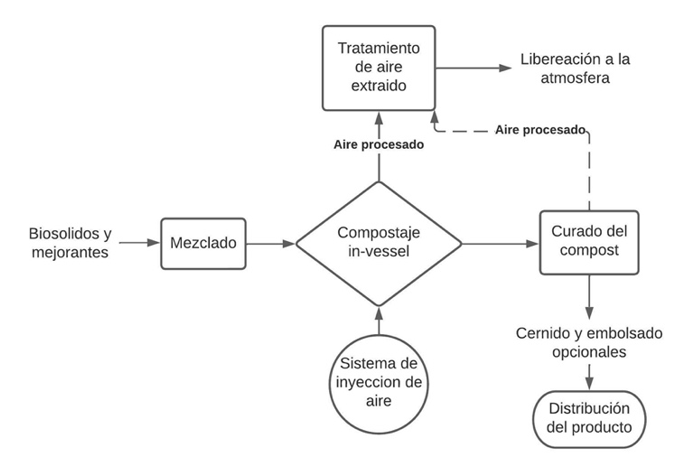
\includegraphics[scale=0.5]{images/Capitulo 1/1.2.1 Marco teorico/Proceso In vessel.png}
            \caption{Diagrama de flujo de una instalación típica de compostaje In-vessel \cite{EPA2020}}
            \label{fg:Invessel}
        \end{figure}

\subsection{Digestión aeróbica}

Consiste en la descomposición biológica de la materia orgánica en presencia de oxígeno, el cual puede ser aportado mediante agitación. Los microorganismos encargados del proceso necesitan aireación para realizar sus funciones de manera eficaz y confiable. Como consecuencia, se obtiene una reducción de olores y volumen de fangos. \cite{SULZER2015}

\subsection{Sistema de agitación}

Este sistema realizará el volteo de la materia orgánica, así como la mezcla de los materiales mientras se genera el proceso de fermentación de las sustancias biológicas. De esta manera, se busca obtener un producto homogéneo a través de los microorganismos que generan los nutrientes.

Esta tarea se puede efectuar a través de diversos tipos de herramientas, cada una adaptada a ciertas características y funciones específicas. \cite{INOX2019} (Tabla \ref{tab:agitacion})


\begin{table}
    \centering
\caption{Tipos de agitadores}
\label{tab:agitacion}
\resizebox{16cm}{!}{
    \begin{tabular}{|m{2cm}|m{5cm}|m{2cm}|m{2cm}|m{2cm}|m{2cm}|} \hline 
         Tipo&  Descripción&  Tipo de flujo&  Campo del flujo generado&  Velocidad tangencial $m/s$ & Viscosidad del medio $Pa * s$ \\ \hline 
         Palas tipo ancla&  Previene adhesión de materiaes, sus brazos llegan cerca de la pared del contenedor, su forma se puede adaptar a la estructura del tanque y favorece el intercambio de calor.&  Laminar&  Tangencial&  Máximo 2& Máximo 1000\\ \hline 
         Paletas o rejilla&  En forma de malla, trabaja a velocidades bajas en recipientes amplios y bajos. Es para fluidos viscosos, con poco esfuerzo de corte.&  Laminar&  Axial&  De 3 a 15& Menores a 8\\ \hline 
         Hélice&  Trabaja en altas velocidades, ideal para liquidos con baja viscosidad. Utilizada para homogenizar mezclas. Favorece el intercambio de calor.&  Turbulento&  Axial&  & Menores a 8\\ \hline 
         Turbina de hojas planas&  Diseño versatil y simple. El comportamiento del fluido se vuelve muy predecible. Ideal para velocidades muy bajas.&  Turbulento&  Axial&  & Menores a 0.11\\ \hline 
         Turbina de hojas inclinadas&  Las palas tienen una inclinación hacia la dirección del flujo, usualmente está comprendida de 3 palas, se utiliza para homogenizar la mezcla y mejora la transferencia de calor.&  Turbulento&  Axial&  De 3 a 8& Hasta 100\\ \hline
    \end{tabular}
    }
    
\end{table}

\subsection{Sistema de trituración}

Uno de los objetivos principales del proceso de trituración es el de reducir el tamaño de los materiales o ajustarlo a las necesidades del proyecto en el cual se utilizarán. Para ello, se requiere de maquinaria con características y funciones muy particulares. \cite{VISE}

\subsection{Sistema de Control}
La función de este sistema es la de gestionar o regular la forma en que se comporta otro sistema para así evitar un mal funcionamiento; tiene como objetivo asegurar el funcionamiento que permita cumplir con todas las tareas y asignaciones para los que fueron programados.

El sistema de control está formado por un conjunto de dispositivos de diverso orden. Pueden ser elementos eléctricos, neumáticos, hidráulicos, mecánicos, entre otros. Los tipos de elementos están determinados por la función a resolver. \cite{SCONT2020} 

Sistema de control de lazo abierto 

El control de lazo abierto se caracteriza por no incorporar un sistema de medición para evaluar el valor de salida. La regulación se hace de forma manual a partir de la experiencia o de los resultados de mediciones obtenidas previamente. \cite{SINADRIVES}

Sistema de control de lazo cerrado

El control de lazo cerrado aparece ante la necesidad de corregir de forma automática errores existentes en la salida del sistema en comparación con el valor de referencia. Esto genera la necesidad de un nuevo elemento en el sistema, un controlador. Un sensor se encarga de medir los valores a la salida, para después transmitir este valor a la entrada del sistema y, como consecuencia, modificar el sistema para obtener el valor deseado. \cite{SINADRIVES} 

\subsection{Interfaz Humano-Máquina}

Una interfaz humano-máquina (HMI por sus siglas en inglés de Human-Machine Interface) permite la comunicación entre el proceso y los operarios. Funciona como un instrumento que permite al operario manipular los procesos.

La función principal de los HMI es mostrar información sobre el monitoreo del proceso, así como ser capaz de transmitir la información operativa del equipo. También es un método por el cual se pueden controlar los objetivos del proceso.

En pocas palabras, la interfaz HMI es una herramienta que permite operar y observar las tareas que se realizan en algún dispositivo para llevar a cabo algún proceso. \cite{IHM2020}

\newpage